If you haven't downloaded and unzipped \href{https://libaoj.in/courses/2021f/MATH3341/zip/Math.3341.zip}{\texttt{Math.3341.zip}}. Download and unzip it under \verb|H:| (H Drive if you are working on the Remote Lab). Change the current working directory by typing \verb|cd H:\Math.3341\Math.3341.Lab.02| in the Command Window, and type \verb|edit lab_02_script| in the Command Window to edit \verb|lab_02_script.m|.

%---------------------------------------------
\section{1-D Array: Vector}
%---------------------------------------------
\begin{enumerate}[(a)]
  \item Define two evenly spaced row vectors: \verb|vec1| of which elements start from $1$ to $9$ with $9$ entries and \verb|vec2| that is between $18$ and $1$ with step size $-2$ using \verb|linspace| and \verb|colon|, respectively. Then store lengths of \verb|vec1| and \verb|vec2| to \verb|vec1Length| and \verb|vec2Length|.
  \item Calculate the following products:
    \begin{itemize}
      \item Store the product of all elements of \verb|vec1| to \verb|vec1Product|.
      \item Calculate the elementwise product of \verb|vec1| and \verb|vec2|, then assign the result to \verb|vecProduct|.
      \item Calculate the dot product of \verb|vec1| and \verb|vec2| in three ways using \verb|dot|, matrix multiplication, and \verb|sum| with elementwise multiplication. Store the results to \verb|dotProduct1|, \verb|dotProduct2|, and \verb|dotProduct3|.
    \end{itemize}
\end{enumerate}

%---------------------------------------------
\section{2-D Array: Matrix}
%---------------------------------------------
\begin{enumerate}[(a)]
  \item Verify that column sums, row sums, and main diagonal sum of a magic square matrix are equal. Define \verb|mat1| to be a $3 \times 3$ magic square matrix. Calculate the column sums \verb|mat1ColSum|, row sums \verb|mat1RowSum|, main diagonal sum \verb|mat1DiagSum| using \verb|sum|.
  \item Create a $3 \times 3$ matrix \verb|mat2| $= \begin{bmatrix} 1 & 2 & 3 \\ 4 & 5 & 6 \\ 7 & 8 & 9 \end{bmatrix}$ by reshaping \verb|vec1| using \verb|reshape| and \verb|transpose|. Then calculate \verb|matProduct1| which is the product of \verb|mat1| and \verb|mat2| using matrix multiplication, and \verb|matProduct2| using elementwise multiplication. Observe the difference between these two multiplications.
  \item Stack \verb|matProduct1| and \verb|matProduct2|, then assign it to \verb|mat3| of which the size is $6 \times 3$. Compute the sum \verb|sumAll| of all elements of \verb|mat3|, column minimums \verb|mat3ColMin|, and row maximums \verb|mat3RowMax| of \verb|mat3|. Find the row indices \verb|rowIndex| and column indices \verb|colIndex| of entries that are \emph{no greater than} $20$ in \verb|mat3|.
  \item Add three new columns to \verb|mat3|:
    \begin{itemize}
      \item Extract the second column of \verb|mat3| and assign it as the fourth column of \verb|mat3|.
      \item Append the vector \verb|int8(rand(6, 1)) * 255)| to \verb|mat3| by specifying the column index to be \verb|end + 1|.
      \item Use bracket to append the vector \verb|colon(0,36,200)| to \verb|mat3| as the last column.
      \item Check the size of \verb|mat3| and store it to \verb|mat3Size|.
    \end{itemize}
\end{enumerate}

%---------------------------------------------
\section{Array: Char Array vs. String Array}
%---------------------------------------------
\begin{enumerate}[(a)]
  \item Define \verb|helloChar|, \verb|worldChar|, \verb|helloString|, \verb|worldString| to be \verb|'hello '|, \verb|'world'|, \verb|"hello "|, \verb|"world"|, respectively. Concatenate the above strings as below:
    \begin{itemize}
      \item Use bracket to concatenate \verb|helloChar| and \verb|worldChar| horizontally and assign it to \verb|helloWorldChar1|. Repeat this to \verb|helloString| and \verb|worldString|, then store the result to \verb|helloWorldString1|.
      \item Now use \verb|strcat| instead of bracket (use \verb|help strcat| to check out the syntax) to repeat the above. Store the results to \verb|helloWorldChar2| and \verb|helloWorldString2|.
    \end{itemize}
\item Use \verb|class| and \verb|length| to determine the types and lengths of \verb|helloWorldChar1|, \verb|helloWorldChar2|, \verb|helloWorldString1|, \verb|helloWorldString2|. Create variables with suffix \verb|Class| or \verb|Length| to store the corresponding results. For example, the length of \verb|helloWorldChar1| should be stored as \verb|helloWorldChar1Length|.
\end{enumerate}

%---------------------------------------------
\section{Application: Image Processing}
%---------------------------------------------
Next we will process Figure \ref{fig:a} to produce Figure \ref{fig:b} in MATLAB. For this portion, suppress the output if it is more than 10 lines by putting \verb|;| at the end of the statement.
\begin{figure}[!hbtp]
  \centering
  \begin{subfigure}[b]{0.25\textwidth}
    \centering
    
\includegraphics[width=80pt]{../pics/UW_gray.png}
    \caption{\texttt{UW_gray.png}}
    \label{fig:a}
  \end{subfigure}
  \begin{subfigure}[b]{0.25\textwidth}
    \centering
    
\includegraphics[width=80pt]{../pics/UW_gray_new.png}
    \caption{\texttt{UW_gray_new.png}}
    \label{fig:b}
  \end{subfigure}
  \caption{UWyo Logo}
\end{figure}

\begin{enumerate}[(a)]
  \item Read \verb|UW_gray.png| and store it to \verb|uwGray| using \verb|imread|. Check the size of \verb|uwGray| and store the size to \verb|uwGraySize|. Find the maximal eigenvalue of the matrix \verb|double(uwGray)| and store it to \verb|maxEigenvalue|.
  \item Crop the Steamboat out of the logo by extracting a submatrix from \verb|uwGray| which starts from row 1 to row 650 and from column 171 to column 650, and save it to \verb|steamboatLeft|. Flip \verb|steamboatLeft| and store it to \verb|steamboatRight|. Then create \verb|steamboat| by concatenating matrix \verb|steamboatLeft| and \verb|steamboatRight|.
  \item Extracting the name \verb|uwName| from \verb|uwGray| which starts from row 651 to row 960 (with all columns). Stack \verb|steamboat| and \verb|uwName| to create \verb|uwGrayNew|. Check the size of \verb|uwGrayNew| which should be $960 \times 960$. If it is correct, write \verb|uwGrayNew| to a file named \verb|UW_gray_new.png| using \verb|imwrite|. List all the variables in the workspace using \verb|whos|.
\end{enumerate}

% %---------------------------------------------
% \section{Defining Variables}
% %---------------------------------------------
% \begin{enumerate}[(a)]
%     \item Define the variable \verb|old_sin_pi = sin(pi)|, then define \verb`pi = 1.25`, and compute \verb`new_sin_pi = sin(pi)`. Compare \verb|old_sin_pi| and \verb|new_sin_pi|.
%     \item Now define \verb`sin = 2.1`. Use \verb`who` and then \verb`whos` to display the list of your currently used variables. Then, evaluate \verb`sin(pi)` in the \verb|try-catch| block.
%     \item Assign \verb`5 + i`, \verb`6 + j` to \verb`a`, \verb`b`, respectively. Then perform summation to \verb`a` and \verb`b` and assign the result to \verb`c`.
% \end{enumerate}
% %---------------------------------------------
% \section{Arrays: Vectors \& Matrices}
% %---------------------------------------------
% \begin{enumerate}[(a)]
%     \item Use \verb`clear` command to clear the variab:sp les in the Workspace.
%     \item Use \verb`linspace` to create a vector $x$ with 10 entries ranging from $0$ to $2\pi$, then assign the transpose of \verb`x` to the variable named \verb`x_transpose` using either \verb`'` or \verb`transpose`. Then use the function \verb`length` to find the length to \verb`x_transpose`.
%     \item Use either \verb`:` or \verb`colon` to create a column vector \verb`v`, of which the range is from 2 to 25 with step size 2. Then use \verb`reshape` to change \verb`v` to a $3 \times 4$ matrix \verb`V`. Find the size of \verb`V` using \verb`size`.
%     \item Define the following two matrices,
%         $$
%         A =
%         \begin{bmatrix}
%             1 & 2 \\
%             3 & 4 \\
%         \end{bmatrix}, \quad
%         B =
%         \begin{bmatrix}
%             5 & 6 \\
%             7 & 8 \\
%         \end{bmatrix}.
%         $$
%         Then store the result of matrix multiplication \verb`A * B` to \verb`C` and the result of element-wise multiplication \verb`A .* B` to \verb`D`. Observe the difference between these two operations.
%     \item Create a $5 \times 5$ magic square matrix \verb`M`. Extract the submatrix of \verb`M` (from row $2$ to row $4$ and from column $3$ to column $5$), and store the submatrix to \verb`M_submatrix`. Then create a vector \verb`M_last_col` by extracting the last column of \verb|M|.
%     \item Create a $4 \times 4$ identity matrix \verb`I` using \verb`eye`, a $6 \times 3$ all-one matrix \verb`N` using \verb`ones`, a $3 \times 4$ all-zero matrix \verb`O` using \verb`zeros`.
% \end{enumerate}

In the Command Window enter the command \verb`diary('lab_02_output.txt')`, run the script file \verb|lab_02_script.m|, then type \verb`diary off` to store the output to \verb`lab_02_output.txt`. Then upload the script file \verb|lab_02_script.m|, output file \verb|lab_02_output.txt|, and \verb|UW_gray_new.png| to the folder \verb|src| on Overleaf. Next open \verb|body.tex| under the folder \verb|LaTeX|. In the last section of the report, you will reproduce the following using \LaTeX{}. Recompile, and submit the generated \verb|.pdf| file to WyoCourses.
%
\newpage

\section{Basics of \LaTeX{}}
\label{sec:bol}
\subsection{Sine functions}
For given $x \in [0, 2\pi]$ with step size $\pi/12$, we can obtain the evaluations of \eqref{eq:sine} at $x$ (see Table \ref{tab:sine}), and the corresponding plot (see Figure \ref{fig:sine}).

\begin{equation}
  \label{eq:sine}
  \begin{cases}
    y_1 = \sin(x/2) \\
    y_2 = \sin(x)   \\
    y_3 = \sin(2x)
  \end{cases}
\end{equation}
\begin{table}[!hbtp]
\centering
\caption{Sine functions}
\label{tab:sine}
\begin{tabular}{ccrr}
\toprule
        $x$ & $\sin(x/2)$ &   $\sin(x)$ &  $\sin(2x)$ \\
\midrule
$0$      & $0$          & $0$  & $0$ \\
$\pi/2$  & $\sqrt{2}/2$ & $1$  & $0$ \\
$\pi$    & $1$          & $0$  & $0$ \\
$3\pi/2$ & $\sqrt{2}/2$ & $-1$ & $0$ \\
$2\pi$   & $0$          & $0$  & $0$ \\
\bottomrule
\end{tabular}
\end{table}
\begin{figure}[!hbtp]
  \centering
  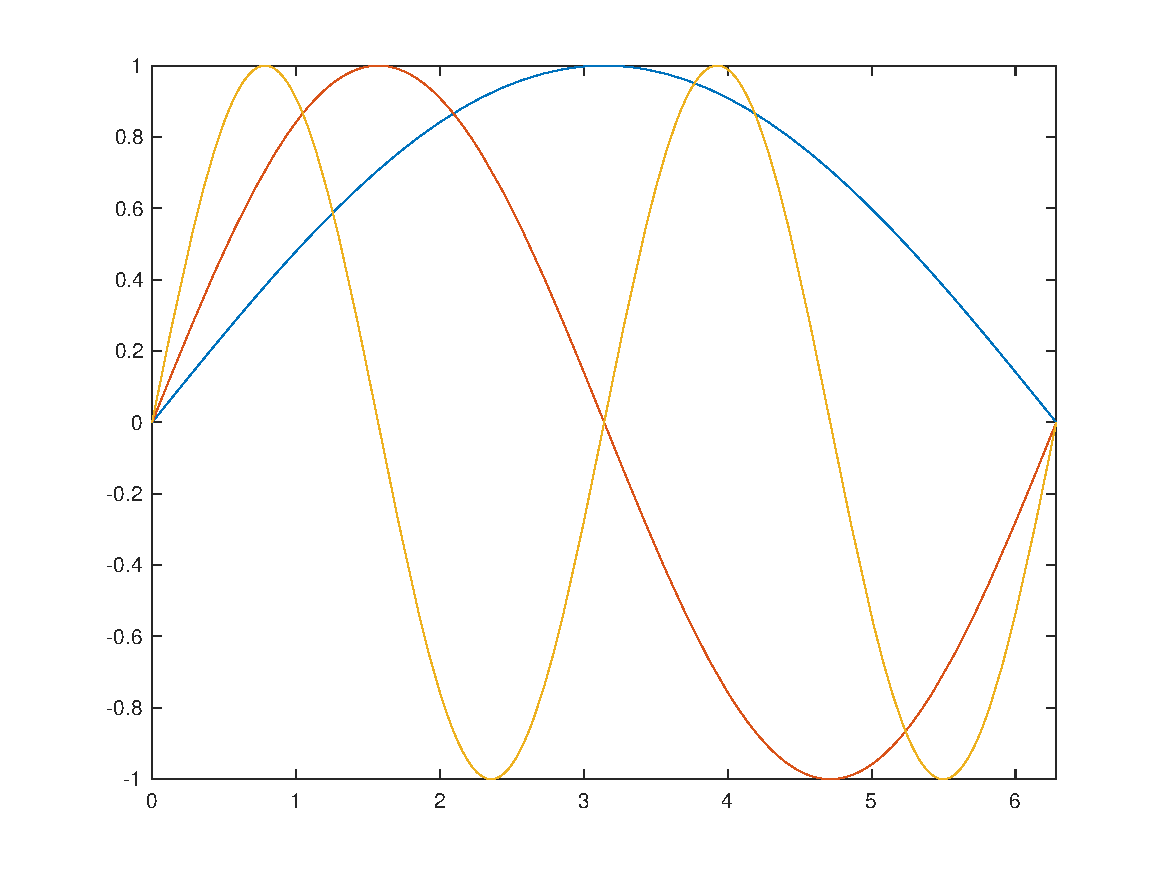
\includegraphics[width=0.3\textheight]{./fig/sine.pdf}
  \caption{Sine functions}
  \label{fig:sine}
\end{figure}

\subsection{Goldbach's Conjecture}
Pursuing this type of analysis more carefully, Hardy and Littlewood in 1923 conjectured (as part of their famous \textsl{Hardy–Littlewood prime tuple conjecture}) that for any fixed $c \geq 2$, the number of representations of a large integer $n$ as the sum of $c$ primes $n = p_1 + \cdots + p_{c}$ with $p_1 \leq \cdots \leq p_c$ should be asymptotically equal to
\begin{equation}
    \label{eq:hardy}
    \left( \prod_{p} \frac{p \gamma_{c,p} (n)}{(p - 1)^c}\right) \int_{2 \leq x_1 \leq \cdots \leq x_c: x_1 + \cdots + x_c = n} \frac{d x_1 \cdots d x_{c - 1}}{\ln{x_1} \cdots \ln{x_c}},
\end{equation}
where the product is over all primes $p$, and $\gamma_{c, p}(n)$ is the number of solutions to the equation $n = q_1 + \cdots + q_c \mod p$ in modular arithmetic, subject to the constraints $q_1, \ldots, q_c \ne 0 \mod p$. This formula \eqref{eq:hardy} has been rigorously proven to be asymptotically valid for $c \geq 3$ from the work of Vinogradov, but is till only a conjecture when $c = 2$. In the latter case, the above formula simplifies to $0$ when $n$ is odd, and to
$$
2 \Pi_2 \left( \prod_{p|n; p \geq 3} \frac{p - 1}{p - 2} \right) \int_{2}^{n} \frac{dx}{(\ln{x})^2} \approx 2 \Pi_2 \left( \prod_{p|n; p \geq 3} \frac{p - 1}{p - 2} \right) \frac{n}{(\ln{n})^2},
$$
when $n$ is even, where $\Pi_2$ is Hardy-Littlewood's twin prime constant
$$
\Pi_2 := \prod_{p \geq 3} \left( 1 - \frac{1}{(p - 1)^2} \right) = 0.6601618158\ldots
$$
This sometimes known as the \textsf{extended Goldbach conjecture}.

\emph{Reference}: \href{https://en.wikipedia.org/wiki/Goldbach's_conjecture}{Goldbach's conjecture}.
